\documentclass[spanish,10pt,a4paper,twoside,openright]{book}

%Informacion
% - Instalar la fuente 'Roboto'


%----------------------------------------------------------------------------------------
%	PAQUETES GENERALES
%----------------------------------------------------------------------------------------
\usepackage[spanish]{babel} 			% Configuracion para palabras en Español (Le quite es-noshorthands)
\usepackage{microtype} 					% Mejor tipografia
\usepackage{amsmath,amsfonts,amsthm} 	% Paquetes para matematicas
\usepackage{graphicx} 					% Requerido para agregar imagenes
\usepackage{float}						% Requerido para el posicionamiento flotante
\usepackage{tcolorbox}					% Permite hacer recuadros para definiciones
\usepackage{multicol}					% Multicolumnas
\usepackage[hidelinks]{hyperref}		% Para el manejo de los hipervinculos
\usepackage{color}						% Permite colocar colores a los textos
\usepackage{circuitikz}					% Permite crear circuitos electricos

%----------------------------------------------------------------------------------------
%	TIPOGRAFIA
%----------------------------------------------------------------------------------------
% OPCION 1 -> Usa la fuente instalada en el sistema
\usepackage{fontspec}						% Configura la fuente. 
\setmainfont{Roboto}						% Para usar Arial, instalar ttf-mscorefonts-installer

% Bloque Inline de Codigo
\definecolor{light-gray}{gray}{0.95}
\newcommand{\code}[1]{\colorbox{light-gray}{\lstinline|#1|}}



%----------------------------------------------------------------------------------------
%	MARGINS AND SPACING
%----------------------------------------------------------------------------------------
\usepackage{geometry}
\geometry{
	top=1cm,
	bottom=1cm,
	left=1cm,
	right=1cm,
	includehead,
	includefoot,
	%showframe, % Descomentar para visualizar los limites
}

% \setlength{\columnsep}{5mm} % Separacion entre columnas
\usepackage{titlesec}						% Permite modificar los espacios de los titulos
\titlespacing{\section}{0pt}{20pt}{5pt}		% Izquierda del titulo, Antes y despues del mismo


\usepackage{afterpage}

\def\blankpage{%
	\clearpage%
	\addtocounter{page}{-1}%
	\null%
	\clearpage}


%----------------------------------------------------------------------------------------
%	ENCABEZADO Y PIE DE PAGINA
%----------------------------------------------------------------------------------------
\usepackage{fancyhdr}	% Permite modificar los Encabezados y Pie de Pagina
\usepackage{lastpage} 	% Used to determine the number of pages in the document (for "Page X of Total")
\fancypagestyle{plain}{
	\fancyhf{}
	\renewcommand{\headrulewidth}{1pt}
	\renewcommand{\footrulewidth}{1pt}
	\fancyfoot[OR, EL]{Pagina \thepage/\pageref*{LastPage}}
	\fancyfoot[OL, ER]{Christian Yoel Herrera}
	\fancyhead[OR, EL]{\textsc{\fecha}}
	\fancyhead[OL, ER]{\tituloHeader}
}

\newcommand{\blankPage}{
	\fancyhf{}
	\renewcommand{\headrulewidth}{0pt}
	\renewcommand{\footrulewidth}{0pt}
	\cleardoublepage
}



%----------------------------------------------------------------------------------------
%	TEXTO EN GENERAL
%----------------------------------------------------------------------------------------
\usepackage{parskip}							% Al usarlo, elimina los espacios entre parrafos
\setlength{\parindent}{0pt} 					% Elimina la sangría
\setlength{\parskip}{6pt plus 1pt minus 1pt} 	% Separacion base: 6pt, Maximo adicional 2pt y minimo adicional 1pt



%----------------------------------------------------------------------------------------
%	FORMATO PARA EL BLOQUE DE CODIGO EN LENGUAJE C
%----------------------------------------------------------------------------------------
\usepackage{listings}	% Permite bloques de codigo

\definecolor{mGreen}{rgb}{0,0.6,0}
\definecolor{mGray}{rgb}{0.5,0.5,0.5}
\definecolor{mPurple}{rgb}{0.58,0,0.82}
\definecolor{backgroundColour}{rgb}{0.95,0.95,0.92}

\lstdefinestyle{CStyle}{
	backgroundcolor=\color{backgroundColour},   
	commentstyle=\color{mGreen},
	keywordstyle=\color{magenta},
	numberstyle=\tiny\color{mGray},
	stringstyle=\color{mPurple},
	basicstyle=\ttfamily\footnotesize,
	breakatwhitespace=false,         
	captionpos=b,                    
	keepspaces=true,                 
	numbers=left,                    
	numbersep=1mm,                  
	showspaces=false,                
	showstringspaces=false,
	showtabs=false,                  
	tabsize=2,
	language=C,
	xleftmargin=3mm, 
	xrightmargin=2mm,
}

\definecolor{codegreen}{rgb}{0,0.6,0}
\definecolor{codegray}{rgb}{0.5,0.5,0.5}
\definecolor{codepurple}{rgb}{0.58,0,0.82}
\definecolor{codeblue}{rgb}{0.2, 0.58, 0.9}
\definecolor{backcolour}{rgb}{0.95,0.95,0.92}

\lstdefinestyle{Matlab}{
	language=Matlab,
	backgroundcolor=\color{backcolour},   
	commentstyle=\color{codegreen},
	keywordstyle=\color{codepurple},
	numberstyle=\tiny\color{codegray},
	stringstyle=\color{codeblue},
	basicstyle=\ttfamily\footnotesize,
	morekeywords={function,writeline,readline,str2double,flush,writeread,split},
	deletekeywords={input},
	morestring=*[d]{"},
	numbers=left,       
	numbersep=-5pt,        
	showstringspaces=false,
	tabsize=2,
	xleftmargin=0.6cm,
	xrightmargin=0.6cm,
	framexleftmargin=10pt,
	framexrightmargin=10pt,
}

\lstdefinestyle{rawStyle}{
	numberstyle=\tiny\color{mGray},
	basicstyle=\ttfamily,
	numbers=left,                    
	numbersep=5pt,                  
	xleftmargin=0.7cm
}




%----------------------------------------------------------------------------------------
%	CONFIGURACION DEL CUERPO (TABLAS Y FIGURAS)
%----------------------------------------------------------------------------------------
\usepackage{booktabs}		% Para centrar las tablas
%\newcommand{\configCuerpo}{
	%	\renewcommand{\figurename}{Figura}
	%	\renewcommand{\tablename}{Tabla}
	%}
\definecolor{GrayCaptions}{rgb}{0.5,0.5,0.5}
\usepackage[
font={color=GrayCaptions},
figurename=Imagen,
tablename=Tabla,
labelfont={it}
]{caption}
\setlength{\abovecaptionskip}{5pt plus 2pt minus 2pt} % Separacion de los 'captions' con el objeto
\setlength{\belowcaptionskip}{5pt plus 2pt minus 2pt} % Separacion de los 'captions' con el texto que continua.





%----------------------------------------------------------------------------------------
%	FORMATO DE LOS CAPITULOS
%----------------------------------------------------------------------------------------
\titleformat{\chapter}[display]
{\normalfont\huge\bfseries}							% Formato general
{\vspace{-2cm}\huge\chaptertitlename\ \thechapter}	% Formato y contenido del subtitulo
{20pt}												% Separacion entre ambos
{\Huge}												% Codigo a ejecutar antes del Subtitulo



%----------------------------------------------------------------------------------------
%	BOXS PERSONALIZADOS
%----------------------------------------------------------------------------------------
\newtcolorbox{boxDef}[1]{
	center,
	width=0.9\textwidth,
	arc=0.2mm,
	boxrule=1pt,
	colframe=black,
	left=3pt,   % Relleno a la izquierda
	right=3pt,  % Relleno a la derecha
	top=3pt,    % Relleno en la parte superior
	bottom=3pt, % Relleno en la parte inferior
	title=#1, 	% Utiliza el argumento para el título
}




%----------------------------------------------------------------------------------------
%	BIBLIOGRAFIA (Para deshabilitar, comentar lo siguiente)
%----------------------------------------------------------------------------------------
\usepackage{csquotes}
\usepackage[
	backend=biber,
	style=apa,
	sortcites,
	url=true
]{biblatex}
\addbibresource{Bibliografia.bib}



\newcommand{\titulo}{Adquisición de Datos - Tektronix TDS360}
\newcommand{\tituloHeader}{Aplicacion para Tektronix TDS360}
\newcommand{\subtitulo}{Diseño de Aplicación en MatLab R2023b}
\newcommand{\autor}{Christian Yoel Herrera}
\newcommand{\fecha}{11 de Marzo de 2025}
\newcommand{\departamento}{Departamento de Electrotecnia}

\usepackage{lipsum}



\begin{document}
	\pagestyle{plain}
	\begin{titlepage}
	\begin{center}
		%---------------------------------------------
		%		LOGO
		%---------------------------------------------
		\vspace*{0.5cm}
		\begin{minipage}{8.0cm}
			\begin{flushright}
				
\includegraphics{images/DobleLogo}
			\end{flushright}
		\end{minipage}
		\begin{minipage}{8.0cm}
			\begin{flushleft}
				\textsc{\huge Universidad Nacional }\\[0.1cm]
				\textsc{\huge de La Plata}\\[0.3cm]
				{\LARGE Facultad de Ingeniería}\\[0.15cm]
				{\Large \departamento}
			\end{flushleft}
		\end{minipage}
		
		\vspace{6cm}
		
		%---------------------------------------------
		%		TITULO & SUBTITULO
		%---------------------------------------------
		\textsc{\Huge \titulo}\vspace{0.5cm}
		\hrule\vspace{0.3cm}
		\textsc{\LARGE \subtitulo}
		
		\vspace{10.0cm}
		
		%---------------------------------------------
		%		AUTOR & FECHA
		%---------------------------------------------
		\textsc{\large \autor}\\[0.1cm]
		\textsc{\textsc{\fecha}}
		
	\end{center}
\end{titlepage}
	\blankPage
	\tableofcontents
	\pagestyle{plain}
	
	% ------------------------> SECCIONES
	\chapter{Introducción}
El osciloscopio de la marca Tektronix, específicamente el modelo TDS 360 permite una comunicación serial utilizando el puerto RS232. Actualmente existen adaptadores de RS232 a USB con lo cual se diseño una aplicación haciendo uso del Software App Designer (de la suite de MatLab) que logre iniciar la comunicación, configurar el osciloscopio y recibir el vector de valores correspondientes a las muestras almacenadas en el registro del Osciloscopio.

\section{Instalación del Driver Prolific}
Dado que Windows instala una versión del driver que no permite hacer uso del adaptador (ya que reconoce que el chip no es original), se deberá instalar el Driver adecuado. Para eso, en la seccion de \textbf{Administrador de Dispositivos}, se debe desinstalar completamente el que instala Windows:

\vspace{5mm}

\begin{center}
	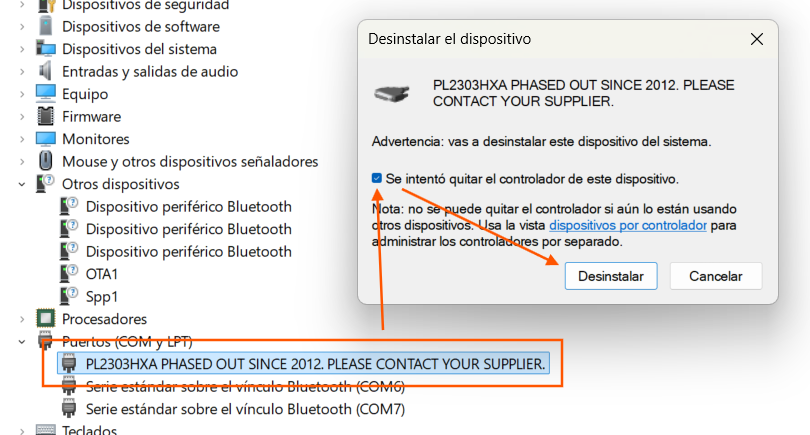
\includegraphics[width=0.8\columnwidth]{images/Driver_01.png}
	\captionsetup{type=figure}
	\caption{Adm. de Dispositivos - Eliminar Driver}
	\label{fig:eliminar-driver}
\end{center}

Luego de este paso, \underline{sin desconectar el adaptador}, se procede a instalar el nuevo driver usando el instalador adjunto al instructivo.

En este punto, si la instalación fue correcta, entonces se utiliza la opción del menú: \textbf{Buscar cambios de Hardware}. En la lista deberá aparecer el nombre:

\begin{center}
	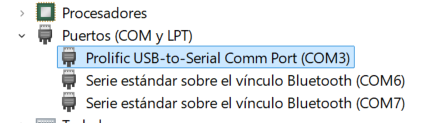
\includegraphics[width=0.45\columnwidth]{images/Driver_02.png}
	\captionsetup{type=figure}
	\caption{Adm. de Dispositivos - Driver Prolific}
	\label{fig:listado-driver-ok}
\end{center}

Si luego de refrescar la lista, sigue apareciendo el driver anterior, se podrá forzar la actualización de la siguiente forma:

\vfill
\newpage

\begin{enumerate}
	\item Seleccionar el elemento de la lista y en las opciones desplegables elegir \textit{Actualizar controlador}.
	\item Seleccionar \textit{Examinar mi PC en busca de controladores}.
	\item Seleccionar \textit{Elegir en una lista de controladores disponibles en el equipo}.
	\item Y de la lista, seleccionar \textbf{Prolific USB-to-Serial Comm Port}
\end{enumerate}

\vspace{5mm}

\textit{\textbf{Nota:} La instalación automatica del driver por parte de Windows se logra porque Windows Update está habilitado. En caso de requerir desactivar esta funcionalidad momentaneamente se puede usar el ejecutable \href{https://www.sordum.org/9470/windows-update-blocker-v1-8/}{\underline{Windows Update Blocker v1.8}})}



\section{Requisitos de la Aplicación}
La primera versión que se logro realizar, tiene el siguiente aspecto.
\begin{center}
	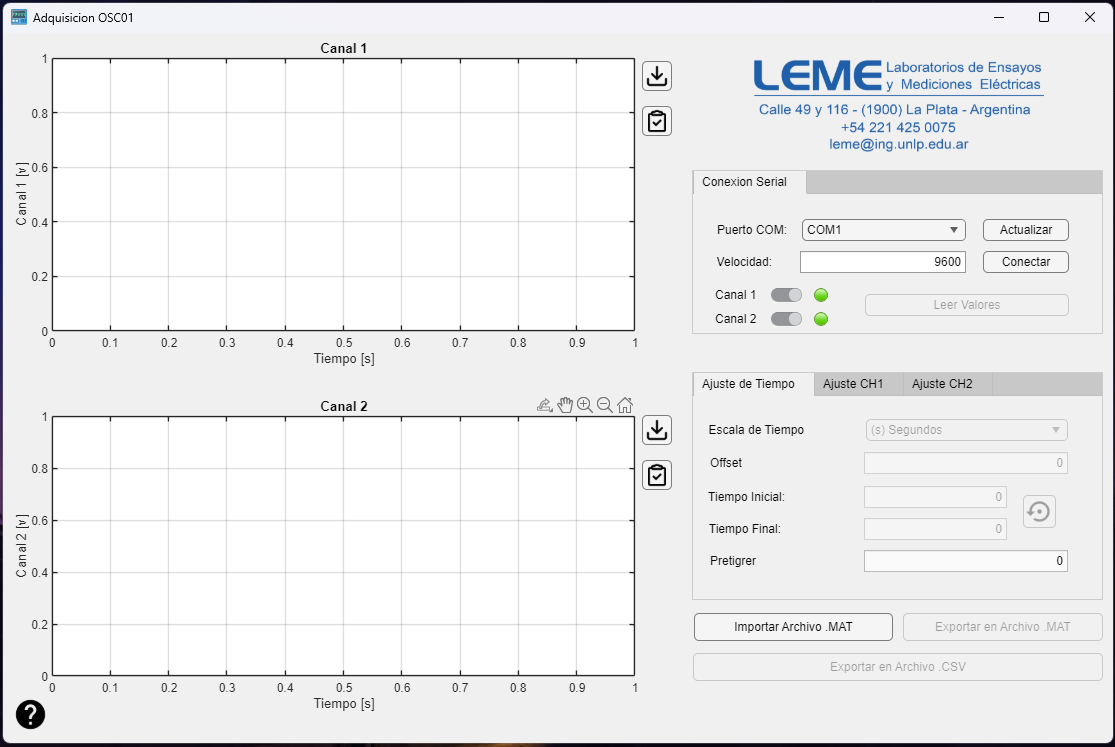
\includegraphics[width=0.8\columnwidth]{images/version_preliminar.png}
	\captionsetup{type=figure}
	\caption{Versión preliminar - Diseño}
	\label{fig:app-pantalla-principal}
\end{center}
El diseño es sencillo, se intenta que disponga de las siguientes funcionalidades:

\begin{itemize}
	\item Que permita configurar los valores esenciales de la comunicación serial, por ejemplo, el puerto \textbf{COM} y los \textbf{Bits por segundo}.
	\item Que verifique la correcta comunicación con el Osciloscopio.
	\item Que luego de solicitar los valores, se disponga de casilleros donde se pueda ajustar los limites de tiempo.
	\item Que los limites del eje vertical de cada canal se pueda modificar.
	\item Que se permita modificar los títulos y las leyendas de cada gráfica.
	\item Que cada canal, disponga de un casillero donde se pueda ingresar un factor, con el fin de aplicar tal valor a cada valor del eje vertical.
\end{itemize}




\section{Comunicación Serial}
En primer lugar, al usar un conversor de RS232 a USB, se procedió a enviar los primeros comandos usando el \textbf{Monitor Serial} del Arduino IDE (Disponible en el \href{https://www.arduino.cc/en/software}{\underline{Link}}).
Los comandos que se usan son los que se enumeran a continuacion. En aquellos donde se especifique \code{CHn}, podra valer \code{CH1} o \code{CH2}.

\begin{itemize}
	\item \code{DATA:ENCDG ASCII}: Configura la codificación de los valores que recibo cuando solicito las muestras almacenadas.
	Esta codificación podrá ser: \code{ASCII}, \code{RIbynary}
	\item \code{HEADER OFF}: Permite que las respuestas no contengan el identificador del comando, de esta forma la respuesta sera unicamente los valores que solicitemos.
	\item \code{DATA:WIDTH 2}: Al configurar en \code{2}, cuando se soliciten las muestras tomadas, el osciloscopio nos devolverá los valores con usando 2 bytes.
	\item \code{DATA:SOURCE CHn}: Permite seleccionar un canal especifico, para luego descargar los valores de este canal.
	\item \code{HORIZONTAL:Main?}: El osciloscopio devolverá el valor de los $^s/_{div}$
	\item \code{CHn:SCALE?}: Permite obtener el valor de los $^v/_{div}$. La elección del canal se hace con \code{CH1} o \code{CH2}.
	\item \code{WFMPRE:CHn:XINCR?}: Permite obtener el valor del tiempo entre dos muestras consecutivas.
	\item \code{WFMPRE:CHn:YMULT?}: Permite obtener el valor por el cual se debe multiplicar cada muestra.
	\item \code{WFMPRE:CHn:YZERO?}: Devuelve el valor del offset vertical.
	\item \code{WFMPRE:CHn:YOFF?}: Devuelve el valor del offset de voltage.
	\item \code{CURVE?}: Al enviar este comando, el osciloscopio devolvera los puntos guardados en su registro, en el formato especificado por \code{DATA:ENCDG}.
	\item \code{HORIZONTAL:TRIGGER:POSITION?}: Es el valor, en porcentaje, de tiempo con respecto a la ventana total de tiempo que se tiene como pre-triger.
\end{itemize}

\vspace{5mm}
El procedimiento para obtener el vector del canal 1 es el siguiente:


\begin{lstlisting}[style=rawStyle]
write("DATA:ENCDG RIBINARY");
write("HEADER OFF);
write("DATA:WIDTH 2");

write("DATA:SOURCE CH1");
write("CURVE?");

xincr = writeread("WFMPRE:CH1:XINCR?");
ymult = writeread("WFMPRE:CH1:YMULT?");
yzero = writeread("WFMPRE:CH1:YZERO?");
yoff  = writeread("WFMPRE:CH1:YOFF?");

adc_raw = readbinblock();
\end{lstlisting}

Finalmente, una vez que se logre recibir el vector de puntos, y los demás valores se procede con la conversión de unidades, con el objetivo de armar los vectores de tiempo y tensión.

\begin{equation}
	volts \;=\; (adc\_raw - y_{off}) \cdot y_{mult} + y_{zero}
	\label{eq:001}
\end{equation}
\begin{equation}
	t \;=\; 0 \;:\; x_{incr} \;:\; (length(volts) - 1) \cdot x_{incr} 
	\label{eq:002}
\end{equation}

La ecuación \ref{eq:002} hace uso de la sintaxis de Matlab, logrando formar un vector desde cero hasta la ultima muestra leida, con un tiempo entre muestra de $x_{incr}$.

Estos comandos fueron los necesarios para descargar todos los valores y datos del canal 1, para hacer uso del canal 2, se repite desde la linea 4 (\texttt{write("DATA:SOURCE CH1);}) haciendo uso del \texttt{CH2}.





	\chapter{Programación en MatLab}
% ------------------------------------------------------------------------------
\section{Funciones Implementadas}
La primer versión usando App Designer, de la suite de MatLab, incorpora funciones que hacen posible el intercambio de información. A continuación se puede ver la versión resumida que permite obtener las muestras. En la aplicación, esto resulta mas complejo ya que se decide si alguno de los canales se deshabilito para su lectura, el control de la ventana de progreso y el manejo de los errores.


\begin{lstlisting}[style=Matlab]
	function LeerValores(app)
		%Leo valores
		flush(app.serial.connection,"input");
		flush(app.serial.connection,"output");
		
		%Solicito los valores de las configuraciones
		app.raw_data.dt = str2double(writeread(app.serial.connection,"WFMPRE:CH1:XINCR?"));
		pp.raw_data.trig_pos = str2double(writeread(app.serial.connection, "HORIZONTAL:TRIGGER:POSITION?"));

		
		%Solicito las muestras del canal 1
		writeline(app.serial.connection,"DATA:SOURCE CH1"); pause(0.5);
		writeline(app.serial.connection,"CURVE?"); pause(0.5);
		ch_t = readline(app.serial.connection);
		app.raw_data.ch1 = str2double(split(ch_t, ","));
		
		%Leo sus configuraciones
		app.raw_data.ch1_mult = str2double(writeread(app.serial.connection, "WFMPRE:CH1:YMULT?"));
		app.raw_data.ch1_zero = str2double(writeread(app.serial.connection, "WFMPRE:CH1:YZERO?"));
		app.raw_data.ch1_off = str2double(writeread(app.serial.connection, "WFMPRE:CH1:YOFF?")); 
		
		%Solicito las muestras del canal 2
		writeline(app.serial.connection,"DATA:SOURCE CH2"); pause(0.5);
		writeline(app.serial.connection,"CURVE?"); pause(0.5);
		ch_t = readline(app.serial.connection);
		app.raw_data.ch2 = str2double(split(ch_t, ","));
		
		%Leo sus configuraciones
		app.raw_data.ch2_mult = str2double(writeread(app.serial.connection, "WFMPRE:CH2:YMULT?"));
		app.raw_data.ch2_zero = str2double(writeread(app.serial.connection, "WFMPRE:CH2:YZERO?"));
		app.raw_data.ch2_off = str2double(writeread(app.serial.connection, "WFMPRE:CH2:YOFF?"));
	end
\end{lstlisting}


Por otra parte, se presenta a continuación la función \texttt{callback} que se ejecuta al presionar el botón conectar.

\begin{lstlisting}[style=Matlab, firstnumber=last]
	function btn_serialConnectButtonPushed(app, event)
		app.serial.connection = serialport(app.dd_serialPort.Value, app.ef_serialBPS.Value, "Timeout", 10);
		
		%Configuro el Encoding y los Bytes
		writeline(app.serial.connection,"DATA:ENCDG ASCII");
		writeline(app.serial.connection,"HEADER OFF");
		writeline(app.serial.connection,"DATA:WIDTH 2");
		
		%Verifico que sea el modelo correcto
		resp = writeread(app.serial.connection, "ID?");
		if ~strcmp(strip(resp, 'right'), "ID TEK/TDS 360,CF:91.1CT,FV:v1.09")
			e.message = 'Erro, el ID no corresponde al Osciloscopio TDS360';
			e.identifier = 'Serial:IDError';
			error(e);                        
		end
	end
\end{lstlisting}

El resto de la programación no es relevante en cuanto a la comunicación con el osciloscopio, por tal motivo se adjunta al documento, un archivo .zip con la versión editable de la misma.

% ------------------------------------------------------------------------------
\section{Configuración en el Osciloscopio}
El osciloscopio tiene el menú para configurar los parámetros de la comunicación serial, la aplicación esta desarrollada para comunicarse con los mismos parámetros que tiene de fabrica el osciloscopio, por tal motivo si hubiera problemas en la comunicación, no siendo una motivo la velocidad de transmisión, entonces se podrá ajustar la configuración de fabrica y asi resolver el inconveniente.










	\chapter{Manual de la Aplicacion}
% ------------------------------------------------------------------------------
\section{Conexión USB}
Como se menciono en las secciones anteriores, se requiere el adaptador RS232-USB, por tal motivo se adjunta el driver correspondiente a el modelo utilizado en el Laboratorio.

Al abrir la aplicación se tiene la sección de \textbf{Conexión}, Después de seleccionar el puerto COM y la Velocidad de Transmisión correspondiente al Osciloscopio, si se presiona \textbf{Conectar} se visualizara el siguiente mensaje.


\begin{center}
	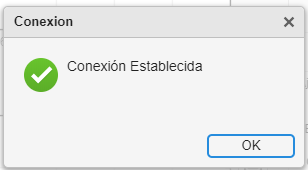
\includegraphics[width=0.3\columnwidth]{images/Conexion_Ok}
	\captionsetup{type=figure}
	\caption{Cuadro de dialogo - Conexión Exitosa}
	\label{fig:002}
\end{center}

En este momento, el bus de datos no se encuentra ocupado, simplemente configuro el Encoding y luego verifico el modelo del osciloscopio. Ahora se permite leer los valores del osciloscopio.

Al presionar \textbf{Leer Valores} realizara la rutina desarrollada en la sección anterior. Lee los parámetros correspondiente al tiempo, luego el canal 1 junto con sus parámetros y por ultimo el canal 2 con sus parámetros. Finalmente, la aplicación armara el vector de tensión, y con la cantidad de puntos leídos estará en condiciones de armar el vector de tiempo.

En caso de existir algún error en la comunicación o en los datos, se visualizara en pantalla con un mensaje indicando el mismo.


\begin{center}
	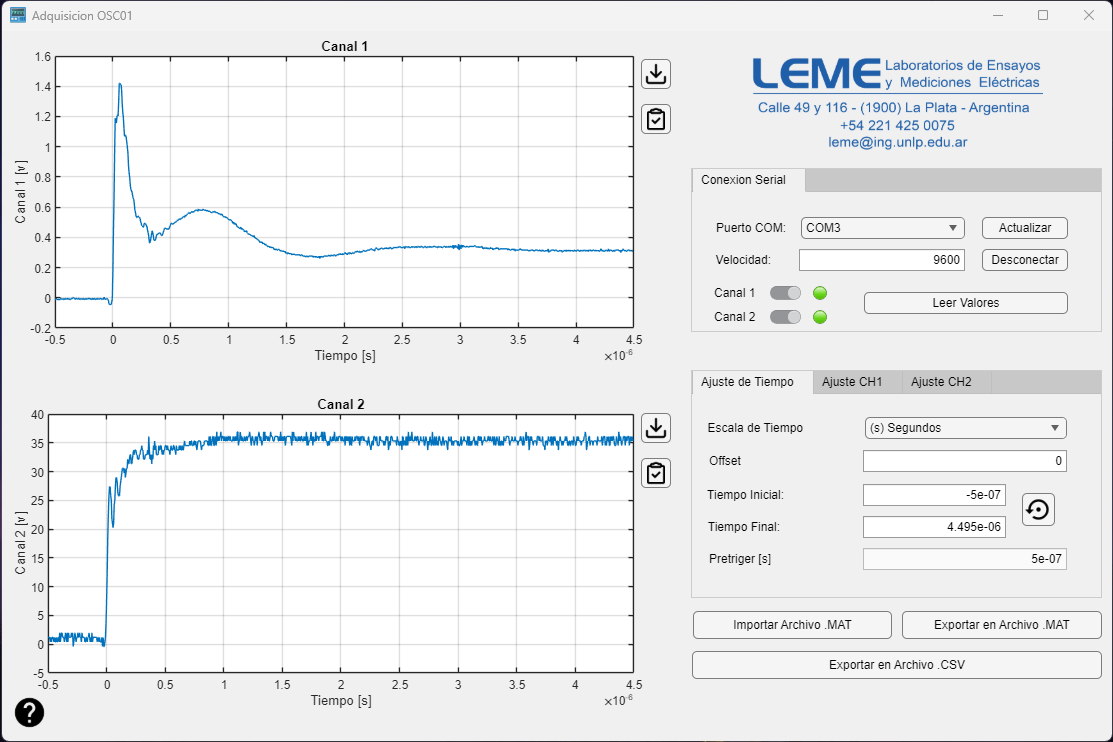
\includegraphics[width=0.7\columnwidth]{images/Datos_Leidos}
	\captionsetup{type=figure}
	\caption{Descarga correcta de valores}
	\label{fig:003}
\end{center}

Una vez leído los valores y presentados en los ejes correspondientes, se habilitan los controles correspondiente al tiempo, y a los volts en cada canal.



\subsection{Ajustes de Tiempo}
La sección de Ajustes de Tiempo permite cambiar las unidades de la escala de tiempo, de esta forma se elimina el multiplicador $x10^{-6}$ como se ve en la imagen \ref{fig:003}.

\begin{center}
	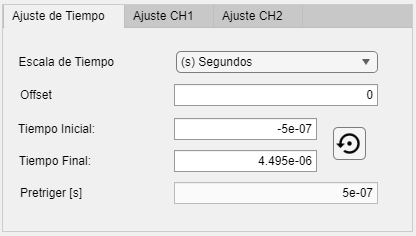
\includegraphics[width=0.4\columnwidth]{images/Ajuste_Tiempo}
	\captionsetup{type=figure}
	\caption{Control de ajustes de tiempo}
	\label{fig:004}
\end{center}

Ademas, se permite configurar un Offset de tiempo, en las unidades elegidas en el selector. Esto permite desplazar el valor de tiempo cero con el fin de anular el tiempo del pre-triger, o bien simplemente desplazar el eje de tiempo.

Los dos campos de \textbf{Tiempo Inicial} y \textbf{Tiempo Final} permiten acotar la ventana de tiempo, con el fin de poder dejar visible una ventana de tiempo especifica. En caso de requerir restaurar la ventana al tiempo que muestreo el osciloscopio, se utiliza el boton para restablecerlo, ubicado entre los dos campos nombrados.

Finalemente, el ultimo campo no es editable y simplemente deja visualizar el valor de tiempo que dura el pre-triger, es decir, sera el tiempo transcurrido entre la primer muestra y el disparo del triger.


\subsection{Ajustes de los Canales}

Al igual que los ajustes de tiempo, se permite ajustar algunos parámetros de las gráficas de cada canal. Los primeros dos, \textbf{Titulo} y \textbf{Etiqueta} son los textos que aparecerán en las gráficas, siendo esto de ayuda para el momento en que se deba exportar la imagen para algún informe.

\begin{center}
	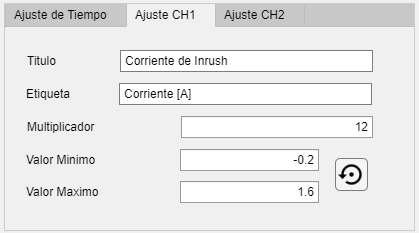
\includegraphics[width=0.4\columnwidth]{images/Ajuste_Canal1}
	\captionsetup{type=figure}
	\caption{Control de ajustes de tiempo}
	\label{fig:005}
\end{center}

El \textbf{Multiplicador} permitirá aplicar un factor por el cual se multiplica cada elemento del vector de tensión correspondiente al canal de la ficha seleccionada.

Los valores de \textbf{Valor Mínimo} y \textbf{Valor Máximo} simplemente ajustan los limites del eje vertical con el fin de dar libertad al momento de exportar la imagen. También se dispone del botón que permite restablecer y ajustar los limites a la amplitud de la curva.

En el Canal 2, se dispone de los mismos parámetros, siendo aplicados a la grafica inferior.

\section{Exportar en Archivo .MAT} \label{Exportar en Archivo .MAT}

El archivo \code{.mat} es propio de MatLab y permite que desde el propio software se puedan leer las variables para lograr manipular o trabajar con estas muestras leídas.

Para generar este archivo, simplemente se presiona el botón \textbf{Exportar en Archivo .MAT}. Se abrira una ventana donde se ubicara seleccionara la ruta y el nombre del mismo, logrando así generar el archivo en cuestión.

Para no modificar la información que se leyó, se devuelve la siguiente estrura de datos:

\begin{itemize}
	\item \code{dt}: Es el valor de tiempo entre muestras.
	\item \code{offset_t}: Es el desplazamiento que se realiza por el usuario en el vector tiempo.
	\item \code{ch1}: Contiene los datos del canal 1, los cuales seran:
	\begin{itemize}
		\item \code{ch1.raw}: Sera el vector que contiene la totalidad de las muestras leidas, correspondientes al canal 1.
		\item \code{ch1.ymult}: Es el factor por el cual se debera multiplicar cada muestra.
		\item \code{ch1.yoff}: Es el valor que se le debera restar al valor RAW leido (antes de usar el multiplicador).
		\item \code{ch1.yzero}: Es el valor de tensión que se le deberá sumar al valor ya convertido en tensión.
		\item \code{ch1.titulo}: Corresponde al texto usado en el titulo de la gráfica.
		\item \code{ch1.leyenda}: Corresponde al texto usado en la leyenda del eje vertical.
	\end{itemize}
	\item \code{ch2}: Se repite la misma estructura que en \code{ch1}.
\end{itemize}

Para lograr usar estos valores en matlab, se puede implementar el siguiente script:

\begin{lstlisting}[style=Matlab, firstnumber=1]
	load('NombreArchivo.MAT');
	
	t = (0:dt:(length(ch1.raw) - 1)*dt) - trig_pos;
	ch1_v = (ch1.raw - ch1.yoff) .* ch1.ymult + ch1.yzero;
	
	plot(t, ch1 .* ch1.factor)
\end{lstlisting}

De esta forma, en MatLab tendremos ahora el vector \code{t} y el vector \code{ch1_v}, los cuales representan el tiempo y los volts (del canal 1). El valor del factor que se utilizo como multiplicador se almacena en \code{ch1.factor}.



\section{Exportar como .CSV}

Para permitir exportar archivos y manipularlos en aplicaciones como Microsoft Excel, se implementa un botón que permite exportarlos con la extensión .CSV. Básicamente hace uso de la funcion \code{writetable()} de MatLab, la cual esta configurada para que guarde unicamente 3 columnas:

\begin{itemize}
	\item \code{Tiempo}: Es el valor del tiempo para cada muestra descargada.
	\item \code{CH1}: Serán las muestras, en Volts del canal 1.
	\item \code{CH2}: Al igual que el anterior, serán las muestras, en Volts del canal 2.
\end{itemize}

Por ultimo, el delimitador se configuro en \textbf{tabs}.


\section{Importar archivo .MAT}
La importación de estos archivo permite que vuelva a visualizar la curva que se encontraba almacenada en el archivo .MAT, de esta forma se podria modificar los valores de los campos disponibles y volver a guardar en un archivo nuevo, o bien como alternativa para editar y luego sobrescribir el archivo.

Para esto, la aplicación dispone del botón \textbf{Importar Archivo .MAT}, la cual primero verificara que las variables mencionadas en la sección \ref{Exportar en Archivo .MAT} estén todas contenidas en el archivo. Si se cumple esta condición, entonces se cargaran los vectores y los valores, completando así en cada campo el valor correspondiente.






\section{Exportar Imágenes}
Para esta funcionalidad, se dispone de dos métodos:

\begin{center}
	
\includegraphics[width=0.06\columnwidth]{images/Boton_ExportImage}
	\captionsetup{type=figure}
	\caption{Botones para exportar imagen}
	\label{fig:006}
\end{center}

El primero corresponde permite \textbf{Descargar} como un archivo de imagen, mientras que el segundo permite \textbf{Copiar} al portapapeles. Como se vera a continuación, cada uno de ellos permitirá elegir la extensión de la imagen.



\subsection{Exportar como Archivo de Imagen}
Al presionar el primer botón, aparecerá un cuadro de dialogo que permitirá seleccionar si el archivo se exportara como imagen vectorial (PDF), o simplemente como una imagen (PNG).
\begin{center}
	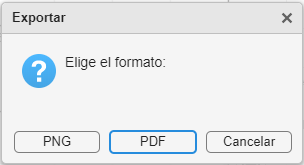
\includegraphics[width=0.4\columnwidth]{images/Export_ImageFile}
	\captionsetup{type=figure}
	\caption{Selección del Formato}
	\label{fig:007}
\end{center}

Luego de la selección, se solicitara la ruta y el nombre del archivo que se exportara.


\subsection{Exportar al Portapales}
Al presionar el segundo botón, aparecerá un cuadro de dialogo que permitira seleccionar si el archivo se copiara como imagen vectorial (SVG), o como simplemente imagen (PNG).

\begin{center}
	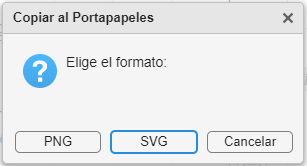
\includegraphics[width=0.4\columnwidth]{images/Export_Clipboard}
	\captionsetup{type=figure}
	\caption{Selección del Formato}
	\label{fig:008}
\end{center}

Luego de la selección, simplemente usar la imagen como si de un texto copiado se tratase.


























	% -----------------------------------
	
	



	% Bibliografia
	%\nocite{*}	% Incorpora todas las referencias, aunque no esten citadas
	%\printbibliography[title={Bibliografia}, heading=bibintoc]
	
\end{document}